\documentclass[11pt,letterpaper]{article}
\usepackage[lmargin=1in,rmargin=1in,bmargin=1in,tmargin=1in]{geometry}
\usepackage{style/quiz}
\usepackage{style/commands}

% -------------------
% Content
% -------------------
\begin{document}
\thispagestyle{title}


% Quiz 1
\quizsol \textit{True/False}: If $P$ is the proposition $6 < 5$ and $Q$ is the proposition, ``Earth is a planet,'' then the logical statement $P \to Q$ is false. \pspace

\sol The statement is \textit{true}. QUIZANSWER \pvspace{0.5cm}

% Quiz 2
\quizsol \textit{True/False}: $\neg (P \to \neg Q) \Longleftrightarrow P \wedge Q$ \pspace

\sol The statement is \textit{true}. QUIZANSWER \pvspace{0.5cm}

% Quiz 3
\quizsol \textit{True/False}: The logic associated to the circuit shown below is the proposition $(\neg P \wedge Q) \vee \neg Q$. \pspace
	\begin{figure}[!ht]
	\centering
	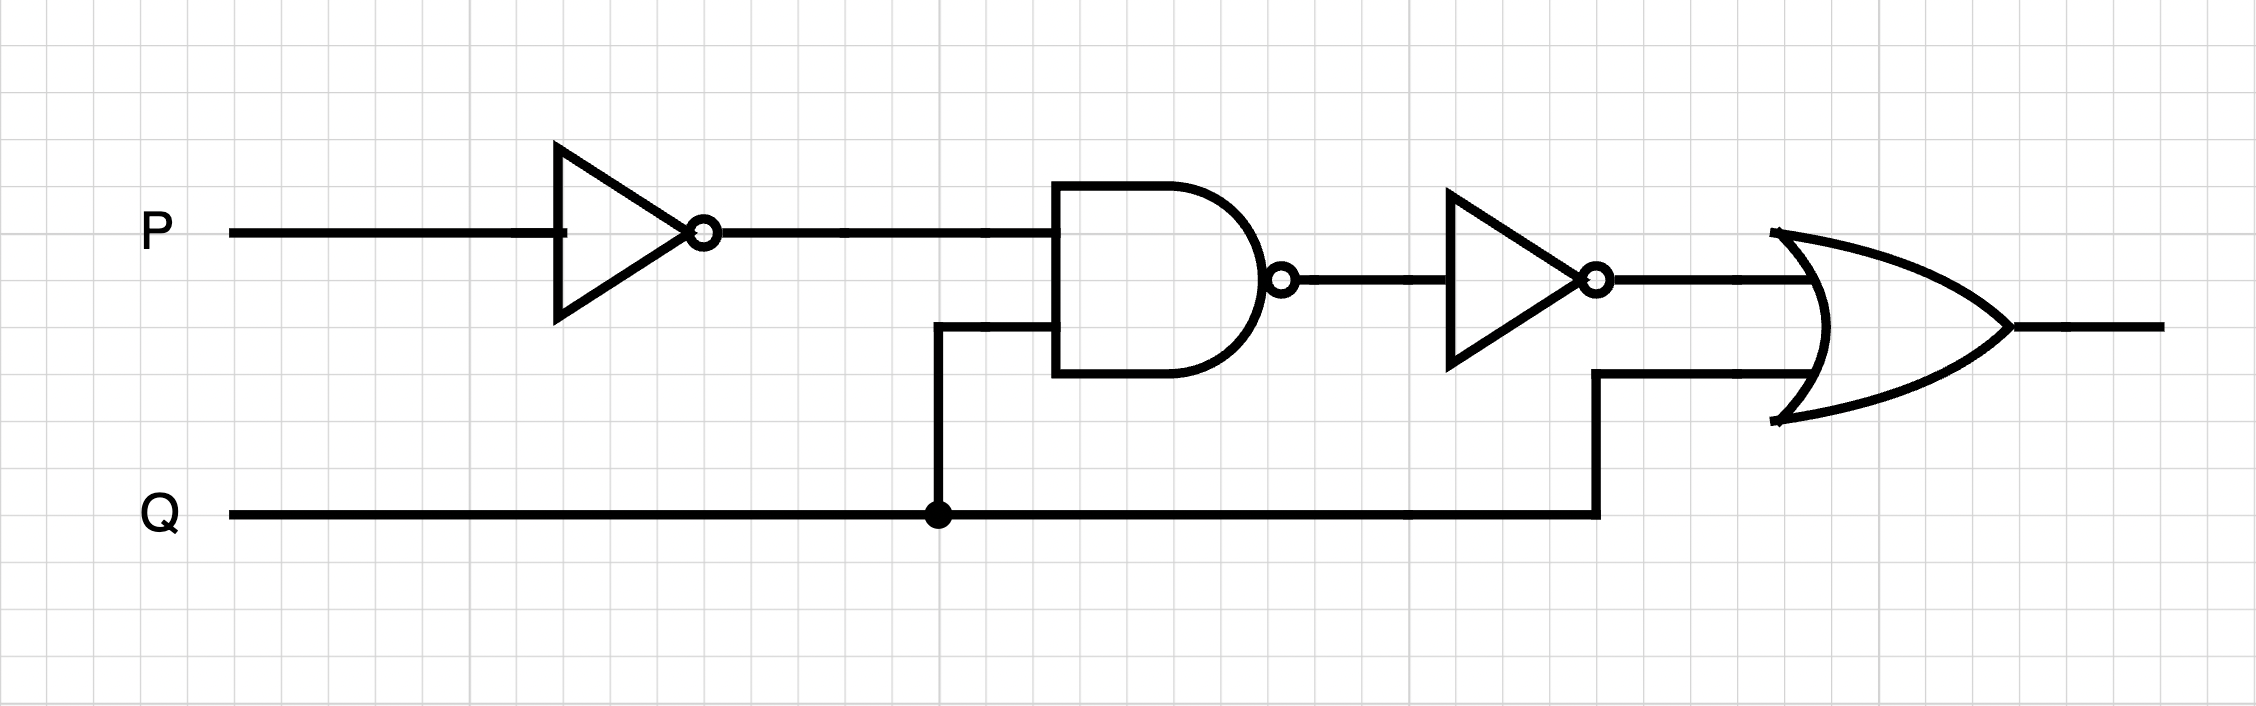
\includegraphics[width=0.75\textwidth]{images/circuit}
	\end{figure} \par

\sol The statement is \textit{true}. QUIZANSWER \pvspace{0.5cm}




% Quiz 4
\quizsol \textit{True/False}: Let the universe $\mathcal{U}$ be the set of real numbers and define $P(x)$ to be the predicate $P(x): x^2 + x - 4 \geq 0$. Then $(\forall x) \big(\neg P(x) \big)$ is true. \pspace

\sol The statement is \textit{true}. QUIZANSWER \pvspace{0.5cm}





\end{document}